
% !TeX spellcheck = en_US
\documentclass{article}
\usepackage[english]{babel}
\usepackage[utf8]{inputenc}
\usepackage{fancyhdr}
\usepackage{xcolor}
\usepackage{lmodern}
\usepackage{listings}
\usepackage{amsmath}
\usepackage{graphicx}
\usepackage{physics}
\lstset{language=[90]Fortran,
	basicstyle=\ttfamily,
	keywordstyle=\color{blue},
	commentstyle=\color{green},
	morecomment=[l]{!\ }% Comment only with space after !
}
\usepackage{color}
\definecolor{deepblue}{rgb}{0,0,0.5}
\definecolor{deepred}{rgb}{0.6,0,0}
\definecolor{deepgreen}{rgb}{0,0.5,0}

% Default fixed font does not support bold face
\DeclareFixedFont{\ttb}{T1}{txtt}{bx}{n}{10} % for bold
\DeclareFixedFont{\ttm}{T1}{txtt}{m}{n}{10}  % for normal

% Python style for highlighting
\lstset{
	language=Python,
	basicstyle=\ttm,
	otherkeywords={self},             % Add keywords here
	keywordstyle=\ttb\color{deepblue},
	emph={__init__},          % Custom highlighting
	emphstyle=\ttb\color{deepred},    % Custom highlighting style
	stringstyle=\color{deepgreen},
	frame=tb,                         % Any extra options here
	showstringspaces=false            % 
}





\pagestyle{fancy}
\fancyhf{}
\lhead{Vincenzo Maria Schimmenti - 1204565}
\rhead{\today}
\rfoot{Page \thepage}
\lfoot{Exercise 7}
\title{%
	Information Theory and Computation \\
	Exercise  7}
\author{Vincenzo Maria Schimmenti - 1204565}

\usepackage{hyperref}

\begin{document}
\maketitle
 
\section*{Theory}
Suppose we want to propagate the wavefunction according to some (possibily time dependent) Hamiltonian $H(t)$. For a small time interval the propagator is:
\begin{equation}
	U(t+\tau,t) \approx e^{-\frac{i}{\hbar}H(t) \tau}
\end{equation}
Since the Hamiltonian is $H=\frac{p^2}{2m}+V(x,t)$ we can use use the BCH formula and split the evolution operator as:
\begin{equation}
	e^{-\frac{i}{\hbar}\hat{H}(t) \tau} = e^{-\frac{i}{\hbar}\frac{\hat{V}(x,t)}{2} \tau} e^{-\frac{i}{\hbar} \frac{\hat{p}^2}{2m} \tau}  e^{-\frac{i}{\hbar}\frac{\hat{V}(x,t)}{2} \tau} +o(\tau^2)
\end{equation}
Now if we have the wavefunction at time $t$, $\ket{\psi(x,t)}$ and we want to apply the evolution operator we may proceed in the following way: we apply first, in space representation, the operator $e^{-\frac{i}{\hbar}\frac{\hat{V}(x,t)}{2} \tau}$; then, by means of Fourier Transform, we represent the result in momentum space, which makes $e^{-\frac{i}{\hbar} \frac{\hat{p}^2}{2m} \tau}$ diagonal. After applying it, we go back to space representation and we apply the last operator. 
\section*{Code Development}
In our task we had to evolve using the time dependent Hamiltonian:
\begin{equation}
	H=\frac{p^2}{2m}+\frac{1}{2} m \omega^2 \left(x-\frac{t}{T}\right)^2
\end{equation}
the ground state of the Harmonic Oscillator $\ket{\psi_0}$. First of all we used the subroutine \textbf{zheev} from \textbf{lapack} in order to diagonalize the Hamiltonian and compute the ground state, for which we used a lattice of spacing $a=0.01$ going from $-5.0$ to $5.0$ and  $\hbar=1.0$, $m=1.0$, $\omega=1.0$. As mentioned in the first section, we used the split operator method to propagate in time the function; the implementation has been done with the following code
\begin{small}
\begin{lstlisting}[language=Fortran]
factor = complex(0, -0.5*tGrd%a*4*acos(-1.0)/(hbar*m*(grd%a*grd%sz)**2))
psi(:,1)=psi0

call dfftw_plan_dft_1d(planf,grd%sz,temp,temp2,FFTW_FORWARD,FFTW_ESTIMATE);
call dfftw_plan_dft_1d(planb,grd%sz,temp2,temp,FFTW_BACKWARD,FFTW_ESTIMATE);

temp = psi0
t = 0.0
do idx=2, tGrd%sz
! potential part, first half
call propagate_hov_shifted(temp,grd,tGrd%a/2,hbar,m,omega,t,Tmax)
! momentum space
call dfftw_execute_dft(planf,temp,temp2)
! multiply by kinetic term
do jdx=1,grd%sz/2
temp2(jdx)=temp2(jdx)*exp(factor*jdx*jdx)
end do

do jdx=1+grd%sz/2, grd%sz
temp2(jdx)=temp2(jdx)*exp(factor*(grd%sz-jdx)**2)
end do
! position space	
call dfftw_execute_dft(planb, temp2, temp)
! potential part, second half
call propagate_hov_shifted(temp,grd,tGrd%a/2,hbar,m,omega,t,Tmax)
psi(:,idx)=temp/grd%sz
temp = psi(:,idx)
t = t + tGrd%a
end do
\end{lstlisting}
\end{small}
In the code \textit{grd} and \textit{tGrd} are custom types characterizing respectively the space grid and the time grid; the subroutine \textit{propagate\_hov\_shifted} multiplies the wavefunction by the potential part of the evolution operator (i.e. by $e^{-\frac{i\tau}{2}V(x,t)}$). The subroutine \textit{dfftw\_plan\_dft\_1d} is internal of \textbf{fftw} and prepares the system for using the Discrete Fourier Transform while \textit{dfftw\_execute\_dft} computes it: we use it twice, once forward and once backward and, in the middle, we multiply by the kinetic part of the evolution operator, i.e. $e^{-i\tau \frac{p^2}{2m}}$ which, again, is diagonal in momentum space. The library \textbf{fftw} stores in the first half of the transformed wave function the positive momentum component while in the second half, reversed, the negative ones; if we denote the momenta as $p_j=\frac{2\pi}{2La \hbar} j$ (with $2L$ the global system size, $N$ the number of points and $a$ the lattice spacing), we will find first the momenta $p_0, \dots, p_{N/2-1}$ and then $p_{-1} \dots p_{-N/2}$.
\newpage
\section*{Results}
Below we show three instants of the wavefunction evolution using its squared norm:
\begin{center}
	\begin{figure}[h!]
		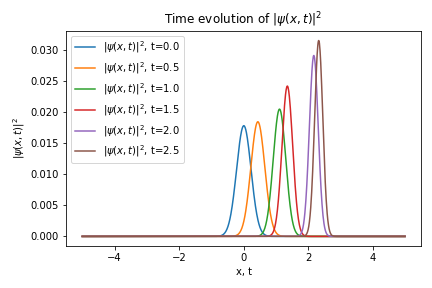
\includegraphics[height=0.5\linewidth]{sqwave.png}
	\end{figure}
\end{center}
We can really appreciate the time evolution if we look at the average position of the particle:
\begin{center}
	\begin{figure}[h!]
		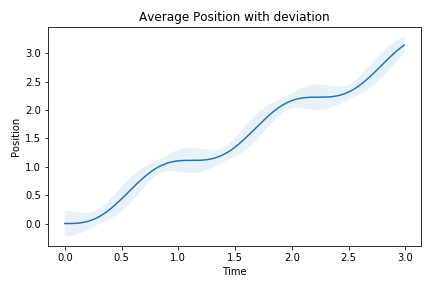
\includegraphics[height=0.5\linewidth]{avgdev.png}
	\end{figure}
\end{center}
This result recalls the classical case of an harmonic particle in a moving frame with constant velocity: its position fluctuates according to a sinusoidal wave with resting point given by $\frac{t}{T}$.
\end{document}